In order to formulate an optimization problem which, when solved, yields 
an optimal mesh triangulation based on representation deficit, a local 
optimization approach~\cite{nocedal_wright_book} is used. Such a 
formulation comes much more naturally than does a formulation based on 
global optimization~\cite{global_optimization_book} when the 
mesh operations defined in Section \ref{sec:meshoperations} are 
employed. One reason for this is the variety of mesh operations that are 
performed at different stages in the mesh generation process; they 
naturally lend themselves to the formulation of different (but related) 
optimization problems as opposed to one unified optimization problem.

It should also be noted that global optimization algorithms are typically 
not used to solve optimization problems with a large number of variables 
-- even if the problem is formulated as a global optimization problem. 
Since there are typically millions to billions of nodes and elements in 
meshes from application problems of interest, a global optimization 
problem would be impractical solve based on the huge number of variables 
that it would necessarily contain. In addition, any global optimization 
problem which would be formulated as a generalization of the local 
optimization problems in this work would be a continuous optimization 
problem. Typically global optimization methods are designed for use on 
discrete optimization problems or on contious optimization problems with 
convex objective functions with guaranteed global minima.

For the above reasons, iterative refinement (a local optimization 
approach) is used to find optimal substructures at each stage of the mesh 
generation process. The local optimization technique employed is
motivated by a class of optimization methods called pattern search 
techniques~\cite{patternsearch1}. Pattern search and multidirectional 
search techniques were developed by Park and Shontz for mesh quality 
improvement~\cite{patternsearch4}; their techniques were based on the 
underlying classes of optimization methods in the literature. Pattern 
search methods do not use derivatives and hence can be used on problems for 
the most general problems for which derivatives either do not exist or are 
impractical to compute.

The optimization employed here uses a simple ``cross'' pattern (up down
left right center, \Cref{crossPattern}) which is sized based on the
local geometry so that it could be moved inside of the triangles/hulls
many times before encountering the boundary. In the case of triangle
splitting, the cross was sized as $0.001$ multiplied by the average edge
length of the triangle. In the case of node movement, the cross was
sized as $0.001$ multiplied by the average edge length of the
topologically attached edges. The cross pattern was not resized during
optimization.  Additionally, the search was not allowed to create
inverted elements.  This was enforced by halting a search whose next
step would create any overlapping edges, tangled elements, etc... Care
was taken to ensure that convergence of the local optimization method
was obtained; this is important since criteria must be met in order for
the heuristic pattern search methods to
converge~\cite{patternsearch2,patternsearch3}.

\begin{figure}
  \begin{center}
  \label{crossPattern}
  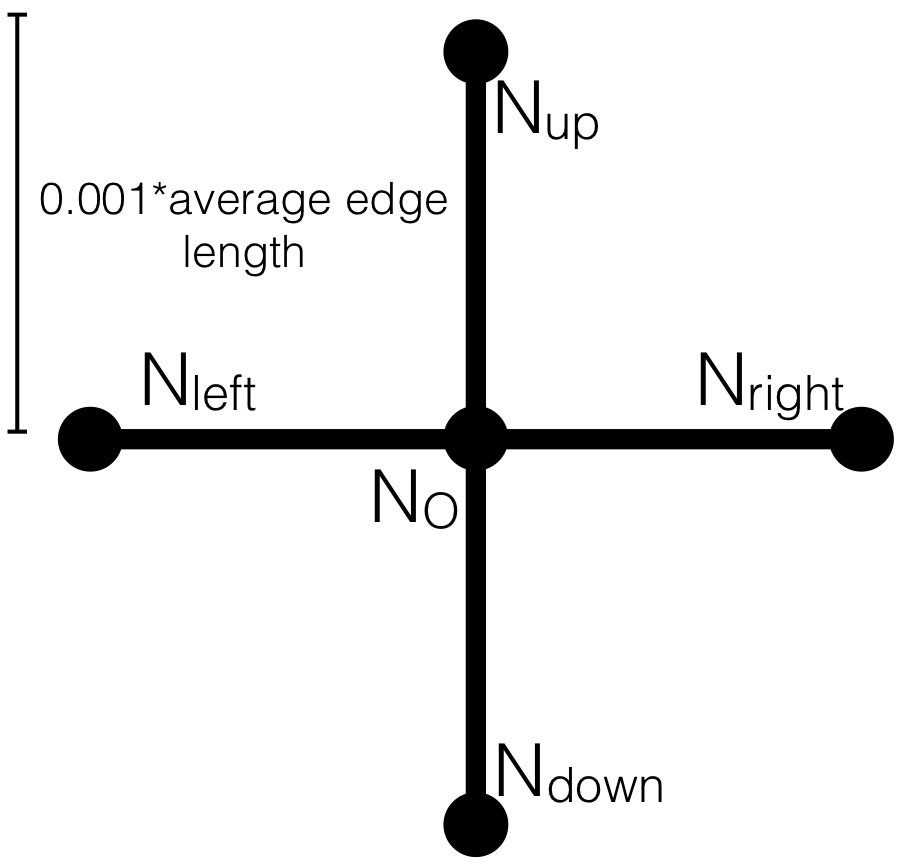
\includegraphics[width=50mm]{Figures/crossPattern.png}
  \caption{Cross Pattern used for Pattern Search Optimization}
  \end{center}
\end{figure}
